
\documentclass[a0paper,portrait]{baposter}

\usepackage{relsize}
\usepackage{bbding}
\usepackage{pifont}

\usepackage[utf8]{inputenc} %unicode support
\usepackage[T1]{fontenc}
\usepackage{amsmath,amssymb,graphicx}
\usepackage[spanish, es-tabla]{babel}    \spanishdecimal{.}
\usepackage{float}
\usepackage{physics}
\usepackage{pifont}

\usepackage[dvipsnames]{xcolor}
\usepackage{setspace}
\usepackage{mwe} % new package from Martin scharrer
\usepackage{tikz,pgfplots}


\usepackage[font=tiny,labelfont=bf]{caption}
\usepackage[theorems,skins]{tcolorbox}

\usepackage{xcolor}
\definecolor{bluemath}{rgb}{0, 1, 0}
\definecolor{blueUNAM}{RGB}{0,60,113}
\definecolor{orangemath}{rgb}{1, .5, .5}
\definecolor{lblue}{RGB}{134,165,169}
\definecolor{bluenice}{RGB}{23,176,199}
\definecolor{gris}{RGB}{118,118,118}
\definecolor{botwgreen1}{RGB}{83,111,80}	
\definecolor{botwgreen2}{RGB}{146,197,130}	
\definecolor{mxpink}{RGB}{229,0,92}	
\definecolor{greenMathematica}{rgb}{0.560181, 0.691569, 0.194885}
%\selectcolormodel{cmyk}
\definecolor{darkgreen}{cmyk}{0.8,0,0.8,0.45}
\definecolor{lgreen}{cmyk}{0.8,0,0.8,0.25}

\graphicspath{{figures/}} % Directory in which figures are stoorange

\newcommand*\tick{\item[\color{mxpink}  \blacksquare ]}
\newcommand{\compresslist}{%
	\setlength{\itemsep}{0pt}%
	\setlength{\parskip}{1pt}%
	\setlength{\parsep}{0pt}%
}

\begin{document}
	\typeout{Poster rendering started}
	\background{ }
	\begin{poster}{
			columns = 4, 
			grid=false,
			headerborder=open, % Adds a border around the header of content boxes
			colspacing=.5em, % Column spacing
			bgColorOne=white, % Background color for the gradient on the left side of the poster
			bgColorTwo=white, % Background color for the gradient on the right side of the poster
			borderColor=white,%darkgreen, % Border color
			headerColorOne= blueUNAM, % Background color for the header in the content boxes (left side)
			headerColorTwo= bluenice, % Background color for the header in the content boxes (right side)
			headerFontColor=white,%white, % Text color for the header text in the content boxes
			%headershade= shade-tb, %plain
			boxColorOne=white, % Background color of the content boxes
			textborder=none, %rectangle, % Format of the border around content boxes, can be: none, bars, coils, triangles, rectangle, rounded, roundedsmall, roundedright or faded
			eyecatcher=true, % Set to false for ignoring the left logo in the title and move the title left
			headerheight=0.09\textheight, % Height of the header
			headershape=rectangle, % Specify the rounded corner in the content box headers, can be: rectangle, small-rounded, roundedright, roundedleft or rounded
			headerfont=\Large\textsf, % Large, bold and sans serif font in the headers of content boxes
			%textfont={\setlength{\parindent}{1.5em}}, % Uncomment for paragraph indentation
			linewidth=2pt % Width of the border lines around content boxes
		}
		%
		%----------------------------------------------------------------------------------------
		%	TITLE AND AUTHOR NAME
		%----------------------------------------------------------------------------------------
		%%
		{
\includegraphics[width=2.7cm]{logo_unam}
			
		} 
		{%Titulo
			\vspace{0.05em}\huge{\color{blueUNAM}{ %Sans Serif
					{\noindent 
						Localización espectral de resonancias plasmónicas en nanoesferas tipo Drude de tamaño arbitrario }}}
		}
		{%Autores
			\normalsize\vspace{0.5em}\\ 
			{\color{mxpink}\textbf{Luna González, Dana L.$^1$}}, Urrutia Anguiano, Jonathan A.$^2$  y Reyes Coronado, Alejandro$^3$
			\vspace{0.3em}\\
			\footnotesize{Departamento de Física, Facultad de Ciencias, Universidad Nacional 	Autónoma de México
				\vspace{0.2em}\\
				$^1$dana.larissalg@ciencias.unam.mx, $^2$jaurrutia.95@ciencias.unam.mx, $^3$coronado@ciencias.unam.mx}
		}
		{
\includegraphics[width=2.85cm]{logo_ciencias}
		} %the author(s)     
		\vspace*{-10cm} 
		\headerbox{ \textbf{ Resumen}}{name=abstract,column=0,row=0, span=4}{\footnotesize 
			La {\color{mxpink}\textbf{nanoplasmónica}} es el estudio de la respuesta electromagnética en sistemas con respuesta metálica a la nanoescala, es decir, con dimensiones menores a 100 nm. En sistemas espacialmente confinados a esta escala, se presenta el fenómeno de {\color{mxpink}\textbf{resonancia de plasmón de superficie localizado}}, resultado del acoplamiento entre los electrones libres de un metal con el campo electromagnético incidente que ilumina al sistema. Este fenómeno se puede emplear en aplicaciones como la espectroscopía y la medicina, debido a la sintonización de dichas resonancias a una frecuencia específica según las propiedades morfológicas del sistema. En este trabajo, se estudia teórica y numéricamente la localización espectral de las resonancias plasmónicas excitadas en {\color{mxpink}\textbf{partículas esféricas}} caracterizadas por una función dieléctrica descrita por el {\color{mxpink}\textbf{modelo de Drude}} en función de su radio.
		}
		%-------Resumen---------------------------
		%-------abstract---------------------------
		
		
		
		%-------Introducción---------------------------
		%-------intro---------------------------
		\headerbox{\textbf{1) Introducción}}{name=intro,column=0,below=abstract,span=2}{\footnotesize 
			La interacción luz-materia puede estudiarse clásicamente mediante la {\color{mxpink}\textbf{absorción}} de parte de la luz incidente en la materia y el {\color{mxpink}\textbf{esparcimiento}} de luz por la materia en todas las direcciones, cuyo efecto combinado resulta en la {\color{mxpink}\textbf{extinción}} del rayo incidente \cite{Bohren}. En los últimos años, en muchos campos de la ciencia aplicada y la tecnología, se han estudiado las propiedades ópticas de partículas de diferentes formas y tamaños , en particular se ha estudiado la dependencia de la sección transversal de extinción del tamaño de las partículas esféricas para describir muestras coloidales.\\
			\begin{center}
				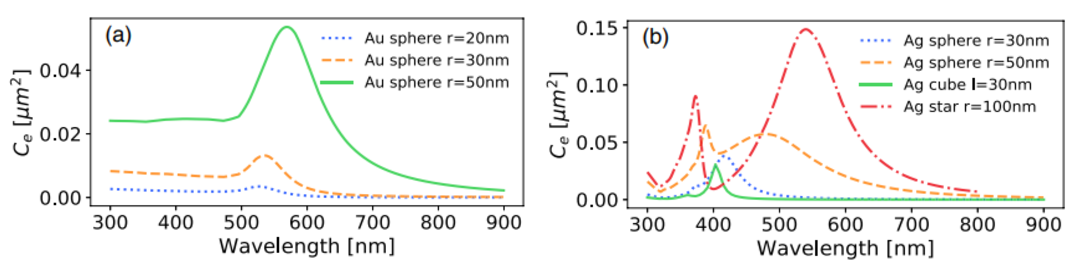
\includegraphics[width=11cm]{Ref.pdf}
			\end{center}
			
			
			El problema de esparcimiento de luz dada una partícula de forma, tamaño y propiedades ópticas específicas iluminada por una onda plana monocromática consiste en conocer los campos electromagnéticos en todos los puntos de la partícula y en todos los puntos del medio homogéneo en el que está embebida \cite{Bohren}.
			
			
		}
		
		
		\headerbox{ \textbf{ Teoría de Mie}}{name=MieTh,column=0,below=intro,span=2}{\footnotesize 
			Al caso particular de esparcimiento por una partícula esférica, la solución a este problema se le conoce como {\color{mxpink}\textbf{teoría de Mie}}. Esta es una solución analítica a las ecuaciones de Maxwell que describe la excitación de la {\color{mxpink}\textbf{resonancia plasmónica de superficie}}  para partículas metálicas esféricas iluminadas por una onda electromagnética (EM) plana. Los campos EMs dentro de la partícula y los esparcidos por esta son descritos mediante coeficientes que corresponden a contribuciones multipolares de {\color{mxpink}\textbf{modos eléctricos}} y {\color{mxpink}\textbf{magnéticos}} mejor conocidos como {\color{mxpink}\textbf{coeficientes de Mie}}. En particular, los coeficientes correspondientes al campo esparcido están dados por \cite{Bohren}:\\
			\begin{minipage}[c]{.55\linewidth}
				{\scriptsize
					$$  \tcboxmath[colback=orange!15!white ,colframe=orange,size=title]{a_n=\frac{m\psi_n(mx)\psi_n'(x)-\psi_n(x)\psi_n'(mx)}{m\psi_n(mx)\xi_n'(x)-\xi_n(x)\psi_n'(mx)}, }$$ $$\tcboxmath[colback=bluenice!15!white ,colframe=blueUNAM, size=title]{b_n=\frac{\psi_n(mx)\psi_n'(x)-m\psi_n(x)\psi_n'(mx)}{\psi_n(mx)\xi_n'(x)-m\xi_n(x)\psi_n'(mx)}, }$$ 
					con $\psi_n(\rho)=\rho j_n(\rho)$ y $\xi_n(\rho)=\rho h_n^{(1)}(\rho)$ las funciones de Ricatti Bessel, $m=n_p/n_m$ y $x=2 \pi n_m/a$ el parámetro de tamaño. }
			\end{minipage}
			\begin{minipage}[c]{.45\linewidth}
				\centering
				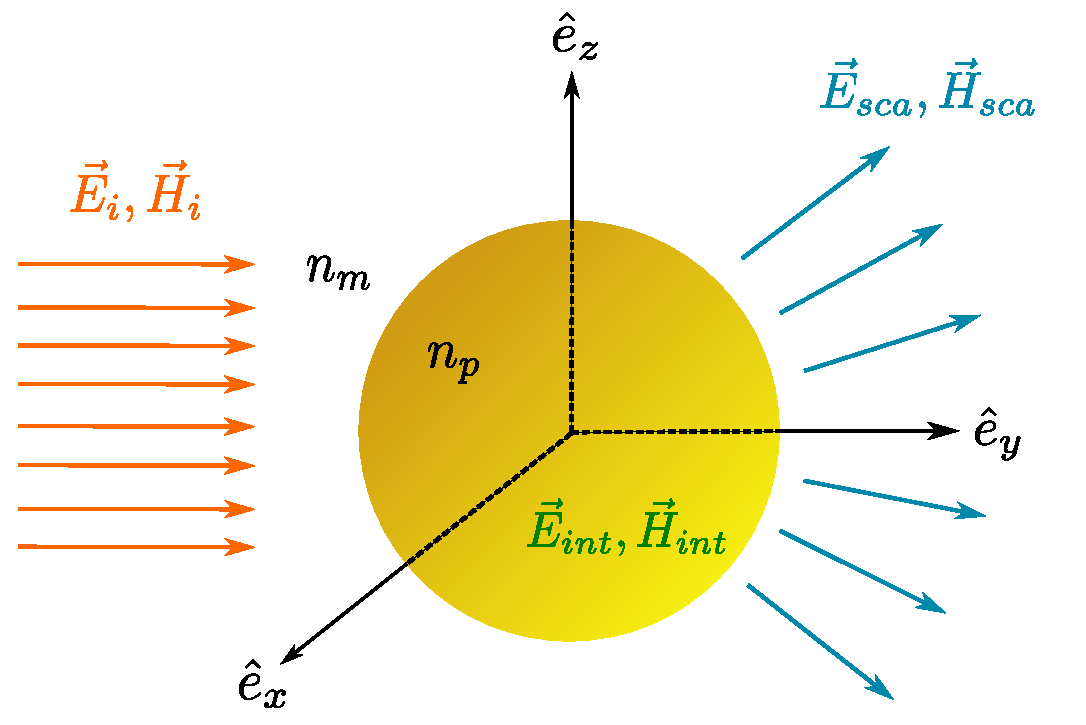
\includegraphics[width=5cm]{scattering.pdf}
				%\captionof{figure}{Partícula de índice de refracción $n_p$ inmersa en un medio de índice de refracción $n_m$. }
				\label{fig:sample_figure}
			\end{minipage}	\\
			
			La {\color{mxpink}\textbf{sección transversal de extinción}} se escribe en términos de los coeficientes de Mie como \cite{Bohren}:
			$$ \tcboxmath[colback=greenMathematica!15!white ,colframe=greenMathematica,size=title]{C_{ext}=\frac{2\pi}{k^2}\sum_{n=1}^{\infty}(2n+1)\text{Re}\{a_n+b_n\}}$$
			cuyo máximo corresponde a la excitación del plasmón de superficie localizado obtenido cuando el denominador  de los coeficientes de Mie es mínimo \cite{Novotny}.\\
			
		}
		
		
		%-------CSM---------------------------
		%-------csm---------------------------
		\headerbox{\textbf{2) Materiales plasmónicos cuando $x\ll 1$}}{name=mdd,column=0,below=MieTh,span=2}{\footnotesize 
			Cuando un material se encuentra en presencia de un campo magnético oscilante, al resolver la ecuación de movimiento que obedecen los electrones libres en el material, se obtiene la {\color{mxpink}\textbf{función dieléctrica tipo Drude}} \cite{Novotny, Ashcroft}
			\begin{equation}
				\tcboxmath[colback=greenMathematica!15!white ,colframe=greenMathematica,size=title]{\frac{\epsilon_D(\omega)}{\epsilon_0} =1-\frac{\omega_p^2}{\omega(\omega+i\gamma)},}
				\label{Drude}
			\end{equation}
			donde $\gamma$ es la constante fenomenológica de amortiguamiento y $\omega_p$ la frecuencia de plasma.\\
			
			Al considerar el {\color{mxpink}\textbf{límite de partícula pequeña}} ($x = k_ma \ll 1$) para esferas inmersas en vacío ($n_m = 1$),  se obtiene que los {\color{mxpink}\textbf{modos normales}} cumplen las relaciones\\
			
			\begin{minipage}[c]{.55\linewidth}
				\centerline{ {\color{orange}\textbf{Eléctricos} } }
				$$\tcboxmath[colback=orange!15!white ,colframe=orange,size=title]{\epsilon_p(\omega_l)=-\frac{l+1}{l},}$$
				Al emplear la Ec.\ref{Drude} y considerar el límite $\gamma\rightarrow0$, al despejar $\omega$ se obtiene 
				$$\tcboxmath[colback=orange!15!white ,colframe=orange,size=title]{\frac{\omega_l}{\omega_p}=\sqrt{\frac{l}{2l+1}}.}$$
			\end{minipage}
			\raisebox{6.5ex}
			{
				\begin{minipage}[b]{.35\linewidth}
					\centerline{ {\color{blueUNAM}\textbf{Magnéticos} } }
					$$\tcboxmath[colback=bluenice!15!white ,colframe=blueUNAM,size=title]{l\stackrel{!}{=}-(l+1), }
					$$  
				\end{minipage}
			}
		}
		%-------CSM---------------------------
		%-------csm---------------------------
		
		%-------modo plasmónico guiado---------------------------
		%-------nmodo---------------------------
		%-------modo plasmónico guiado---------------------------
		%-------nmodo---------------------------
		
		%-------modo plasmónico guiado---------------------------
		%-------nmodo---------------------------
		\headerbox{\textbf{4) Resultados numéricos}}{name=nmodo,span=2,column=2,below=abstract}{\footnotesize
			
			Dado que para partículas de mayor radio, las resonancias deben de calcularse de forma numérica, se empleó el método de la sección dorada [pones referencia]. Se reescribieron $n_p$ y $x$ en términos de variables adimensionales
			$$n_p=\sqrt{1-\frac{1}{\tilde{\omega}(\tilde{\omega}+i\tilde{\gamma})}},\hspace{1cm}x=\tilde{\omega}\tilde{a}n_m.$$	
			donde $\omega_p a/c$ compara la frecuencia de excitación $\omega$ con el	tiempo de acoplamiento $ac^{-1}$ entre la interacción EM de la esfera y la densidad de carga
			inducida que corresponde al plasmón de superficie \cite{Aizpurua}. 
			
			se busca entonces encontra
			
			
			
			
			\begin{tikzpicture}
				\node at (-2.5,5) {\footnotesize \textbf{Eléctricos}};
				\node at (3,5) {\footnotesize \textbf{Magnéticos}};
				\node[inner sep=0pt] (graf) at (0,1){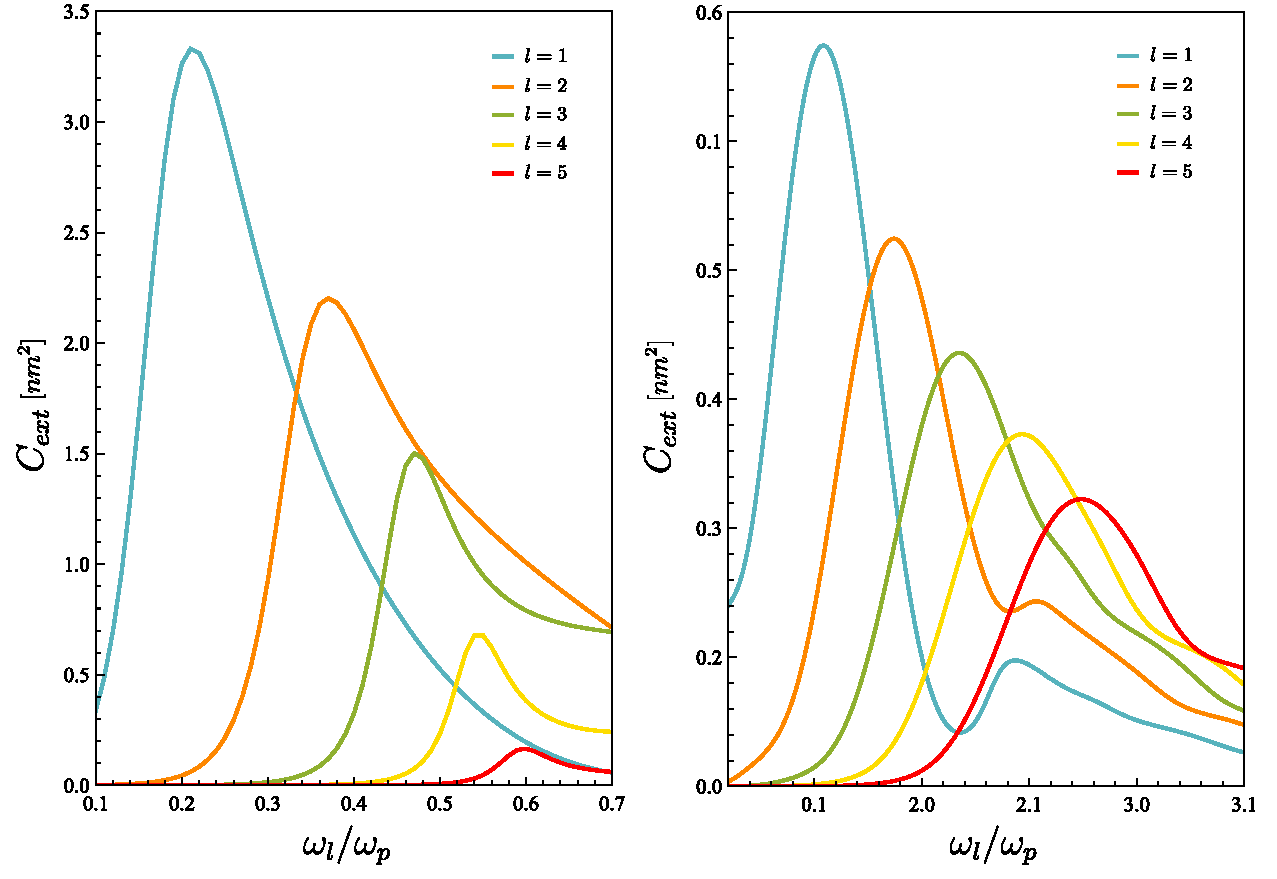
\includegraphics[scale=.5]{SeccTrans2.pdf}};
				\node[inner sep=0pt] (graf) at (0,-4.5){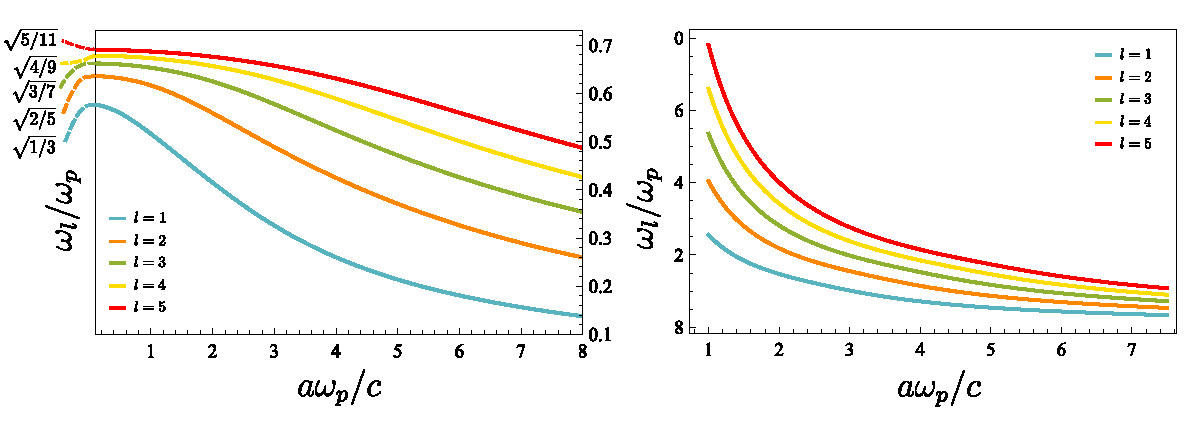
\includegraphics[scale=.57]{Resonances.pdf}};
			\end{tikzpicture}
			
			
		}
		
		\headerbox{\textbf{5) Conclusiones}}{name=conclusiones,column=2,below=nmodo,span=2}{
			\footnotesize
			\begin{itemize}
				\tick La banda de frecuencias en la que las frecuencias de resonancia de los modos eléctricos se espera que se encuentren es $[\omega_{p}/\sqrt{3},\omega_{p}/\sqrt{2}]$, cuyos límites corresponden al modo plasmónico dipolar eléctrico y a la resonancia plasmónica de superficie de una esfera de radio infinito, es decir, a un plano infinito.
				\tick Conforme el límite de partícula pequeña deja de ser válido se presenta un corrimiento al rojo de las resonancias plasmónicas de superficie localizadas de los modos eléctricos y magnéticos para partículas esféricas.
				\tick No es posible calcular una aproximación de las frecuencias de resonancia de los modos normales magnéticos en el límite de partícula pequeña.
			\end{itemize}
		}
		%-------modo plasmónico guiado---------------------------
		%-------nmodo---------------------------
		
		
		
		
		
		\headerbox{\textbf{6) Referencias}}{name=references,column=2,span=2,below=conclusiones}{
			\renewcommand{\section}[2]{\vskip 0.05em} % Get rid of the default "References" section title
			\begin{thebibliography}{99} \scriptsize \compresslist
				\bibitem{Bohren} C.F. Bohren y D.R. Huffman , \textit{Absorption and scattering of light by small particles} (John Wiley \& Sons, 1980). 
				\bibitem{Novotny} L. Novotny, \textit{Principles of Nano-Optics} (Cambridge University Press, New York, 2006). 
				\bibitem{Ashcroft} N.W. Ashcroft y N.D. Mermin, \textit{Solid State Physics}, \textit{Principles of Nano-Optics} (Saunders College, 1976). 
				\bibitem{Aizpurua} J. Aizpurua, \textit{Coupling of electrons and electromagnetic surface modes in scanning transmission electron microscopy} (Tesis doctoral, Universidad de País Vasco, País Vasco, España,
				1998). 
			\end{thebibliography}\footnotesize
		}
		
		\headerbox{{\scriptsize Agradecimientos al proyecto PAPIIT-UNAM IN107122 y a la Facultad de Ciencias de la UNAM}}{name=thaks,column=2,span=2,below=references}{ \hfill}
		
	\end{poster}
	
\end{document}